\documentclass{beamer}
\usepackage[utf8]{inputenc}
\usepackage{amsmath}
\usepackage{amssymb}
\usepackage{tikz}
\usepackage{pgfplots}
\pgfplotsset{compat=1.17}

\usetheme{Madrid}
\usecolortheme{default}

%------------------------------------------------------------
%This block of code defines the information to appear in the
%Title page
\title[MATH 116: Probability] 
{MATH 116: Probability}

\subtitle{Section 8.7}

\author[S. Boardman]
{Sam Boardman}

\date[2/25/26]
{February 25, 2026}

%End of title page configuration block
%------------------------------------------------------------

\begin{document}

%The next statement creates the title page.
\frame{\titlepage}

\begin{frame}{What Is Probability?}
    \begin{itemize}
    
        \item A number between 0 and 1 describing the likelihood of an event

        \vfill
        
        \item To convert to a percentage, multiply by 100
        \begin{itemize}
            \item Example: ``The probability Exam 2 will be on March 23rd is .995"
            \item Equivalently: ``The probability Exam 2 will be on March 23rd is \only<1>{...\%}\only<2->{99.5\%}"
        \end{itemize}

        \vfill 

        \item<3> Need to specify assumptions to calculate probabilities
        \begin{itemize}
            \item Probabilities are not inherently correct or incorrect, just self-consistent 
        \end{itemize}
        
    \end{itemize}
\end{frame}

\begin{frame}[shrink]{Example: Rolling a Die}

    \begin{itemize}
        \item Assumption 1: The die is fair

        \begin{table}[h]
        \small
        \centering
        \begin{tabular}{|c|c|}
        \hline
        Event & Probability \\
        \hline
        Roll 1 & $.1\overline{6}$ \\
        \hline
        Roll 2 & $.1\overline{6}$ \\
        \hline
        Roll 3 & $.1\overline{6}$ \\
        \hline
        Roll 4 & $.1\overline{6}$ \\
        \hline
        Roll 5 & $.1\overline{6}$ \\
        \hline 
        Roll 6 & $.1\overline{6}$ \\
        \hline
        \end{tabular}
        \end{table}

        \item<2-> Assumption 2: The die is lightest on the side marked 1

        \begin{table}[h]
        \small  
        \centering
        \begin{tabular}{|c|c|}
        \hline
        Event & Probability \\
        \hline
        Roll 1 & .7 \\
        \hline
        Roll 2 & .0625 \\
        \hline
        Roll 3 & .0625 \\
        \hline
        Roll 4 & .0625 \\
        \hline
        Roll 5 & .0625 \\
        \hline 
        Roll 6 & .05 \\
        \hline
        \end{tabular}
        \end{table}

        \item<3-> Question: What is wrong with saying ``Rolling each number either happens or it doesn't, so the probability of rolling each number is .5?"
    
    \end{itemize}
\end{frame}

\begin{frame}{What is a Statistic?}
    \begin{itemize}
        \item Statistic: Number that varies randomly

        \vfill
        
        \item Examples of statistics:
        \begin{itemize}
            \item Amount of time (in minutes) someone spends waiting for their bus
            \item Height (in feet) of a person selected from the general population
        \end{itemize}

        \vfill 

        \item In this class: Study statistics that have infinitely many possible values, where each has probability 0
        \begin{itemize}
            \item For instance, the age ``27" represents a bunch of exact ages: 27.0, 27.25, 27.5556, 27.99, 27.999,...
        \end{itemize}

        \vfill

        \item Two equivalent ways to describe a statistic probabilistically:
        \begin{itemize}
            \item Probability density function (PDF)
            \item Cumulative distribution function (CDF)
        \end{itemize}
        
    \end{itemize}
\end{frame}

\begin{frame}{Probability Density Function (PDF)}
    \begin{block}{Probability Density Function (PDF)}
    A probability density function for a statistic is a function $p(x)$ such that \begin{itemize}
        \item $p(x) \geq 0$ for all real numbers $x$; and
        \item $\int_{-\infty}^{\infty} p(x)dx = 1$
    \end{itemize}
    \end{block}

    \begin{itemize}
        \item $p(x)dx$ = infinitely small probability the statistic is equal to $x$
        \item Probability that statistic is between $a$ and $b$ = $\int_a^b p(x)dx$
        \item $\int_{-\infty}^{\infty} p(x)dx = 1$ says that the probability the statistic is equal to something between $-\infty$ and $\infty$ is 1
    \end{itemize}
    
\end{frame}

\begin{frame}{Practical Interpretation of PDFs}

\begin{itemize}
    \item If $c$ is in $[a,b]$, then the probability that statistic is between $a$ and $b$ $$\approx p(c)\cdot(b-a)$$
\end{itemize}


\begin{center}
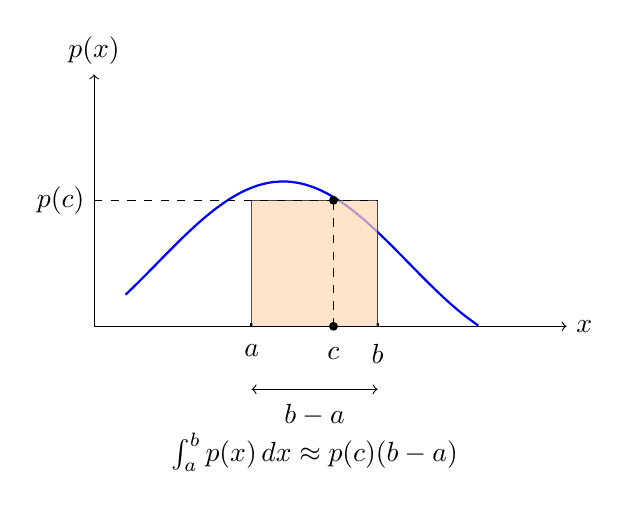
\begin{tikzpicture}[scale=.8]

% Axes (extended x slightly)
\draw[->] (0,0) -- (7.5,0) node[right] {$x$};
\draw[->] (0,0) -- (0,4) node[above] {$p(x)$};

% Interval [a, b] (Moved closer together: a=2.5, b=4.5)
\draw[thick] (2.5,0) -- (2.5,0.05) node[below=4pt] {$a$};
\draw[thick] (4.5,0) -- (4.5,0.05) node[below=4pt] {$b$};

% Function p(x) (Domain extended from 1:6 to 0.5:6.5)
\draw[domain=0.5:6.1, smooth, thick, blue] plot (\x, {1+1.3*sin(45*(\x-1))});

% Rectangle: height at p(c)
% Adjusted coordinates for narrower width and a higher average height visual
% New height chosen visually at y=2.0
\draw[fill=orange!30, opacity=0.7] (2.5,2.0) rectangle (4.5,0);

% Dotted lines for c
% New c chosen at x=3.8 where the curve hits the new height y=2.0
\draw[dashed] (3.8,0) -- (3.8,2.0);
\draw[dashed] (0,2.0) -- (4.5,2.0);

% Point c
\fill (3.8,0) circle (2pt) node[below=4pt] {$c$};
\fill (3.8,2.0) circle (2pt); % top of rectangle

% Labels
% Position updated for new height y=2.0
\node[left] at (0,2.0) {$p(c)$};
\node at (3.5,-2) {$\int_a^b p(x)\,dx \approx p(c)(b-a)$};

% Optional: Indicate the width
% Updated x coordinates from 1 and 6 to 2.5 and 4.5
\draw[<->] (2.5,-1) -- (4.5,-1) node[midway, below=2pt] {$b-a$};

\end{tikzpicture}
\end{center}
    
\end{frame}

\begin{frame}{Cumulative Distribution Function (CDF)}
    \begin{block}{Cumulative Distribution Function (CDF)}
    A cumulative distribution function for a statistic is a function $P(x)$ such that \begin{itemize}
        \item $P$ is increasing: If $a < b$, then $P(a) \leq P(b)$
        \item $\lim_{x \to -\infty} P(x) = 0$
        \item $\lim_{x \to \infty} P(x) = 1$
    \end{itemize}        
    \end{block}

    \begin{itemize}
        \item $P(x)$ = probability the statistic is less than or equal to $x$
        \item $\lim_{x \to -\infty} P(x) = 0$ says that the statistic cannot be equal to $-\infty$ 
        \item $\lim_{x \to \infty} P(x) = 1$ says that the statistic cannot be equal to $\infty$
    \end{itemize} 
    
\end{frame}

\begin{frame}{Translating Between PDFs and CDFs}
    \begin{itemize}
        \item<1-> Suppose a statistic has PDF $p(x)$. How do we obtain its CDF $P(x)$?
        \item<2-> Answer: $P(x) = \int_{-\infty}^x p(t)dt$

        \vfill

        \item<3-> Suppose a statistic has CDF $P(x)$. How do we obtain its PDF $p(x)$?
        \item<4-> Answer: $p(x) = P'(x)$

        \vfill 

        \item<5-> Summary: The CDF is the antiderivative of the PDF such that $\lim_{x \to -\infty} P(x) = 0$
    \end{itemize}
    
\end{frame}

\begin{frame}{Example: Selecting a Random Number in [0,6]}
    \begin{itemize}
        \item Statistic: Number selected
        \item Assumption 1: Each number in [0,6] is equally likely
        \begin{itemize}
            \item PDF: $p(x) = \begin{cases}
                0, & x < 0 \\
                \frac{1}{6}, & 0 \leq x \leq 6 \\
                0, & x > 6
            \end{cases}$ \pause 

            \vfill 
            
            \item CDF: $P(x) = \int_{-\infty}^x p(t)dt$ \pause 
            \begin{itemize}
                \item If $x < 0$, $P(x) = \int_{-\infty}^x 0dt = 0$ \pause 
                \item If $0 \leq x \leq 6$, $P(x) = \int_{-\infty}^0 0dt + \int_0^x \frac{1}{6}dt = 0 + \frac{t}{6}|_0^{x} = \frac{x}{6}$ \pause 
                \item If $x > 6$, $P(x) = \int_{-\infty}^0 0dt + \int_0^6 \frac{1}{6}dt + \int_6^x 0dt = 0 + \frac{t}{6}|_0^{6} + 0 = 1$ \pause
                \item In summary, $P(x) = \begin{cases}
                    0, & x < 0 \\
                    \frac{x}{6}, & 0 \leq x \leq 6 \\
                    1, & x > 6
                \end{cases}$
            \end{itemize}
        \end{itemize}
    \end{itemize}
\end{frame}

\begin{frame}{Example: Waiting Time for a Bus}
    \begin{itemize}
        \item Statistic: Waiting time (in minutes)
        
        \begin{itemize}
            \item PDF: $p(x) = \begin{cases}
                0, & x < 0 \\
                \frac{1}{10}, & 0 \leq x \leq 5 \\
                \frac{1}{10}e^{-(x-5)/5}, & x > 5
            \end{cases}$ \pause 

            \vfill 
            
            \item CDF: $P(x) = \int_{-\infty}^x p(t)dt$ \pause 
            \begin{itemize}
                \item If $x < 0$, $P(x) = \int_{-\infty}^x 0dt = 0$ \pause 
                \item If $0 \leq x \leq 5$, $P(x) = \int_{-\infty}^0 0dt + \int_0^x \frac{1}{10}dt = 0 + \frac{t}{10}\Big|_0^{x} = \frac{x}{10}$ \pause 
                \item If $x > 5$, $P(x) = \int_{-\infty}^0 0dt + \int_0^5 \frac{1}{10}dt + \int_5^x \frac{1}{10}e^{-(t-5)/5}dt$ \\ 
                \qquad \quad \ $= 0 + \frac{1}{2} + \left(-\frac{1}{2}e^{-(t-5)/5}\right)\Big|_5^x = 1 - \frac{1}{2}e^{-(x-5)/5}$ \pause
                \item In summary, $P(x) = \begin{cases}
                    0, & x < 0 \\
                    \frac{x}{10}, & 0 \leq x \leq 5 \\
                    1 - \frac{1}{2}e^{-(x-5)/5}, & x > 5
                \end{cases}$
            \end{itemize}
        \end{itemize}
    \end{itemize}
\end{frame}

\iffalse
\begin{frame}{Sanity Checks}

\begin{center}
\begin{tikzpicture}[scale=.6]
\begin{axis}[
axis x line=middle,
axis y line=middle,
ymin=-0.05, ymax=0.25,
xmin=-2, xmax=8,
samples=200,
ylabel={$p(x)$},
xlabel={$x$},
xtick={0,6},
ytick={1/6},
yticklabels={$\frac{1}{6}$},
width=10cm, height=5cm,
domain=-2:8,
clip=false,
]
% Plot the piecewise function
\addplot [
thick, blue,
samples=2,
domain=-2:0
] {0};

\addplot [
thick, blue,
samples=2,
domain=0:6
] {1/6};

\addplot [
thick, blue,
samples=2,
domain=6:8
] {0};

% Open/Closed Circles at the endpoints
\addplot[blue, fill=white, only marks, mark=*, mark size=2pt] coordinates {(0,0) (6,0)};
\addplot[blue, only marks, mark=*, mark size=1.5pt] coordinates {(0,1/6) (6,1/6)};

\end{axis}
\end{tikzpicture}
\end{center}
    
\end{frame}
\fi

\end{document}